\documentclass{article}
\usepackage[margin=1.0in]{geometry}
\usepackage{tikz}
\usetikzlibrary{fit}
\usetikzlibrary{positioning}
\usetikzlibrary{bending}
\usetikzlibrary {arrows.meta} 
\usetikzlibrary {shapes.symbols} 
\usetikzlibrary {shapes.geometric}
\usetikzlibrary {shapes.multipart} 
% \usetikzlibrary{external}
% \tikzexternalize % activate!
\title{Point Clouds in an N-ary Tree}
\author{Brett Viren}
% \hypersetup{
%  pdfauthor={Brett Viren},
%  pdftitle={},
%  pdfkeywords={},
%  pdfsubject={},
%  pdfcreator={Emacs 28.2}, 
%  pdflang={English}}




\tikzset{
  treenode/.style= {
    circle,
    color = black!30,
    draw,
    fill = yellow!30,
    line width = 1mm,
    inner xsep = 3mm,
    inner ysep = 3mm
  },
  pointcloud/.style= {
    cloud,
    cloud ignores aspect,
    cloud puffs=11,
    color = black!30,
    draw,
    fill = yellow!30,
    line width = 1mm,
    inner xsep = 3mm,
    inner ysep = 3mm
  },
  disjointdataset/.style= {
    rectangle split,
    rectangle split parts=#1,
    rectangle split horizontal,
    draw,
    anchor=center,
  },
  namedpcs/.pic = {
    \node[pointcloud] (-pc1) {``PC1''};
    \node[pointcloud,below=0.0mm of -pc1.mid] (-pc2) {``PC2''};
  }

}

\begin{document}
\maketitle

\section{Point clouds}

In the Wire-Cell toolkit (WCT), a \textbf{point cloud}\footnote{See WCT document Point Cloud for details} is of type \texttt{PointCloud::Dataset} which is effectively a \texttt{std::map<std::string, Array>}.  An \texttt{Array} is contiguous storage with a dynamic numerical type.


\begin{center}
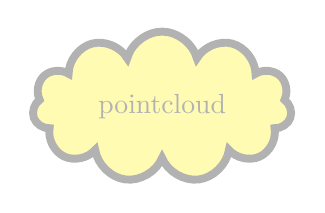
\begin{tikzpicture}
  \node[pointcloud] {pointcloud};
\end{tikzpicture}
\end{center}
We \textbf{aggregate and name} a set of point clouds with a type such as \texttt{std::map<std::string,Dataset>}.

\begin{center}
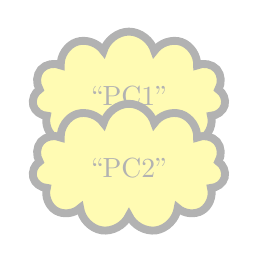
\begin{tikzpicture}
  \pic (pcA)  {namedpcs};
\end{tikzpicture}
\end{center}
Point clouds of similar schema (same \texttt{Array} names and shapes) may sequenced into an \textbf{ordered collection}.  We may \textbf{concatenate} them via the \texttt{Dataset::append() method} producing a larger, monolithic, ``flat'' dataset and incurring a copy.  Or we may keep individual point clouds distinct by producing a sequence of point clouds which are held \textbf{by reference} to avoid the copy.  This can be done using the type \textbf{PointCloud::DisjointDataset}.

\begin{center}
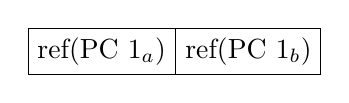
\begin{tikzpicture}[disjointdataset/.style={
    rectangle split,
    rectangle split parts=#1,
    rectangle split horizontal,
    draw, anchor=center}]
  \node[disjointdataset=2] {ref(PC $1_a$)\nodepart{two}ref(PC $1_b$)};
\end{tikzpicture}
\end{center}
Of course, we may combine these two types of aggregations to have named sequences of point clouds, for example with the type \texttt{std::map<std::string, DisjointDataset}.  We will call these collections \textbf{scoped point clouds} and we will call 
collections of type \texttt{std::map<std::string,Dataset>} \textbf{local point clouds}.  The terms ``scoped'' and ``local'' will become clear below after introducing the concept of a \textbf{point cloud tree}.

\section{$n$-ary tree}

Putting aside point clouds for a moment we now describe the basic concepts of $n$-ary tree data structures\footnote{In the context of trees, the term $n$-ary (aka $\{n,m,k\}$-ary) is an extension of the term \textit{binary} that is used for the special case that $n=2$}.  

A tree is an arrangement of general objects called \textbf{nodes}.

\begin{center}
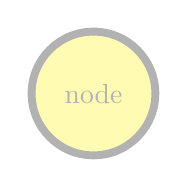
\begin{tikzpicture}
  \node[treenode] {node};
\end{tikzpicture}
\end{center}
A node is an object defined to have \textbf{three parts}.  First, we allow a node to hold a \textbf{value} (aka ``payload'') object of some type.  

\begin{center}
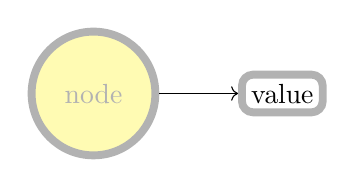
\begin{tikzpicture}
  \node[treenode] (node) {node};
  \node[right=of node,draw=black!30,line width=1mm,rounded corners] (value) {value};

  \draw[->] (node) edge (value);
\end{tikzpicture}
\end{center}
In this and further diagrams, ownership is indicated by a \textbf{solid arrow}.
Next, we allow a node to have \textbf{zero or one parent nodes}.  Equivalently, a node may \textbf{zero or more children nodes}.

In WCT $n$-ary trees, \textbf{nodes own their children nodes} (children are held by \verb|std::unique_ptr<>|) and a node will merely \textbf{reference its parent node} (hold a bare pointer). 
The children are organized into an ordered list so children nodes \textbf{reference their neighboring siblings}.
A tree with three nodes, one parent and two children are illustrated. 
A reference is indicated with \textbf{dashed arrow}.
Again, while only two are drawn, an $n$-ary tree node may have zero or more children.

\begin{center}
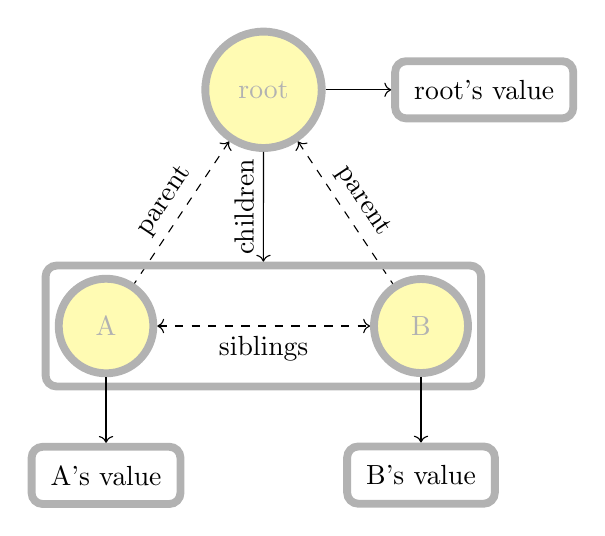
\begin{tikzpicture}[level/.style={sibling distance=40mm/#1}]
  \node[treenode] (r) {root}
  [level distance=30mm]
  child {
    node[treenode] (a) {A}
    edge from parent [<-,dashed]
    node[above,draw=none,sloped] {parent}
  }
  child {
    node[treenode] (b) {B}
    edge from parent [<-,dashed]
    node[above,draw=none,sloped] {parent}
  };
  \draw[dashed,<->] (a) -- node[below]{siblings} (b) ;

  \node[draw=black!30,line width=1mm,rounded corners,fit=(a) (b)] (children) {};
  \draw[->] (r) -- node[above,sloped]{children} (children);

  \node[below=10mm of a] (pcA) {A's value};
  \node[draw=black!30,line width=1mm,rounded corners,fit=(pcA)] (aval) {};
  \draw[->] (a) -- (aval) ;

  \node[below=10mm of b] (pcB) {B's value};
  \node[draw=black!30,line width=1mm,rounded corners,fit=(pcB)] (bval) {};
  \draw[->] (b) -- (bval) ;

  \node[right=10mm of r] (pcR) {root's value};
  \node[draw=black!30,line width=1mm,rounded corners,fit=(pcR)] (rval) {};
  \draw[->] (r) -- (rval) ;

\end{tikzpicture}
\end{center}

As implemented in WCT, \textbf{a tree is just its nodes}. 
There is no ``tree object'' per se. 
Rather, if some code context holds a ``root'' node then that code may access all nodes in the tree. 
Code is free to manually  navigate the child/parent/sibling edges. 
More conveniently forms of \textbf{tree descent iteration} are provided.  

A number of \textbf{depth-first descent} iteration methods are implemented.  A descent may visit a node and all its descendants.  A descent may instead be limited to some maximum depth.  For example a descent on a root note with a depth of unity (1) will visit only that root node.  A descent with a depth of two (2) will visit the root node and its direct children.  A depth of three (3) will also include grandchildren, etc.  The special depth of zero marks unlimited descent.

Negative descent depths are not defined.  However, from any node one may define a \textbf{unique ascending path} from that node to any ancestor node up to and including the root node.  This path is ordered starting with the node of interest.  The \textbf{path length} is comparable to the \textbf{descent depth}.  A path length of one contains only the node of interest, two contains the parent, three the grand parent, etc. 

A node may be removed from the ordered collection of children nodes owned by a parent. 
Any siblings that were previously neighbors to the removed node will themselves become mutual neighbors in the new collection. The removed node then becomes a root node of a tree holding its descendants (if any).

Conversely, a node may of course be added as a child to another node.  In principle, this node may be inserted in an arbitrary location in a node's collection of child nodes but for now we consider only appending.

\section{Point cloud tree}

In WCT, a \textbf{point cloud tree} or \textbf{point tree} is an $n$-ary tree with a \textbf{node value} type that provides storage and management of \textbf{point clouds} and any \textbf{k-d trees} that have been formed on the point clouds. 
This node value type is provided \texttt{PointCloud::Tree::Points}.  An object of this type consists primarily of three parts:

\begin{enumerate}
  \item a set of \textbf{local} named point clouds
  \item a set of \textbf{scoped} point clouds
  \item a set of \textbf{scoped} k-d trees built on the scoped PCs
\end{enumerate}
The term \textbf{local} refers to data that is atomic to the context of the node that provides it while 
\textbf{scoped} data is a composed as a \texttt{DisjointDataset} introduced above.   Scoped data is an important concept for WCT point trees and is described more below.

These three parts of a \texttt{Points} object in relation to its node are illustrated in the following diagram.

\begin{center}
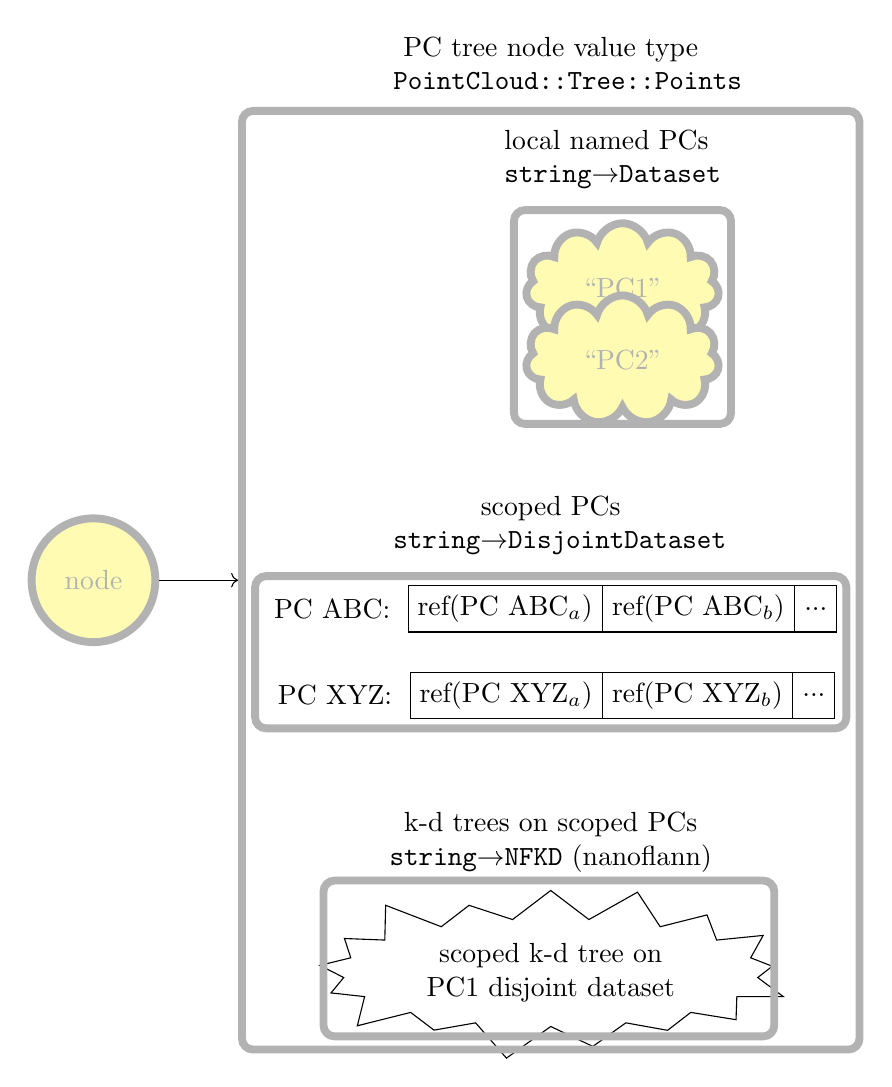
\begin{tikzpicture}[level/.style={sibling distance=40mm/#1}]

  % local PCs
  \pic (pcA) {namedpcs};
  \node[draw=black!30,line width=1mm,rounded corners,fit=(pcA-pc1) (pcA-pc2)] (pcval) {};
  \node[above=1mm of pcval,text width=3cm] (pclab) {local named PCs \texttt{string}$\to$\texttt{Dataset}};
  
  % scoped PCs
  \node[disjointdataset=3,below=20mm of pcval] (djds1) {
    ref(PC ABC$_a$)\nodepart{two}ref(PC ABC$_b$)\nodepart{three}...};
  \node[left=1mm of djds1] (djds1n) {PC ABC:};
  \node[disjointdataset=3,below=5mm of djds1] (djds2) {
    ref(PC XYZ$_a$)\nodepart{two}ref(PC XYZ$_b$)\nodepart{three}...};
  \node[left=1mm of djds2] (djds2n) {PC XYZ:};
  \node[draw=black!30,line width=1mm,rounded corners,fit=(djds1) (djds2) (djds1n) (djds2n)] (djdsval) {};
  \node[above=1mm of djdsval,align=center,text width=4cm] (djds) {scoped PCs \texttt{string}$\to$\texttt{DisjointDataset}};

  % scoped k-d trees
  \node[starburst, draw, below=20mm of djdsval,align=center,text width=3.5cm] (kd) {
    scoped k-d tree on PC1 disjoint dataset};

  \node[draw=black!30,line width=1mm,rounded corners,fit=(kd)] (kdval) {};
  \node[above=1mm of kd, text width=4.5cm,align=center] (kdlab) {k-d trees on scoped PCs \texttt{string}$\to$\texttt{NFKD} (nanoflann)};

  % \draw[dashed,out=45,in=-90,looseness=1,<-] (pcA-pc2) edge (djds.one south);
  % \draw[dashed,out=45,in=-90,looseness=1,<-] (pcB-pc2) edge (djds.two south);
  % \draw[dashed,out=0,in=0,looseness=2,->] (kd) edge (djds.two east);

  \node[draw=black!30,line width=1mm,rounded corners,fit=(kdlab) (kdval) (djdsval) (pcval) (pclab)] (allval) {};
  \node[align=center,above=1mm of allval,text width=4cm] {PC tree node value type \texttt{PointCloud::Tree::Points}};

  \node[treenode,left=of allval] (node) {node};
  \draw[->] (node) edge (allval);

\end{tikzpicture}
\end{center}

\section{Point cloud tree scope}

In WCT point trees, a \textbf{scope} bundles information to describe a selection of a subset of the data in the tree.  Selected data is said to be ``in scope'' with respect to a given node though the scope itself is independent from any particular nodes.  A scope is defined by three items:

\begin{enumerate}
\item A \textbf{depth} limit for a depth-first descent iteration.
\item A \textbf{pcname} of local point clouds.
\item A \textbf{list of array names} of point cloud arrays (in the named point clouds).
\end{enumerate}

A scope may be applied to a point cloud tree to produce a representation of a point cloud called a 
\textbf{scoped point cloud}.  As introduced above, a scoped point cloud is represented by a \texttt{DisjointDataset}.
The construction of the scoped point cloud follows these rules:

\begin{enumerate}
\item A node is provided as the root of the scope.
\item A depth-first descent iteration begins at the root node.
\item The depth of the descent is limited by the scope's \textbf{depth} value.
\item If a visited node lacks a local point cloud with the name given by the \textbf{pcname} it is ignored and the iteration continues.
\item If a visited node lacks an array for each in the \textbf{list of array names} an exception is raised.
\item The node is now considered to be ``in scope'' and the arrays named by the \textbf{list of array names} from the local point cloud given by \textbf{pcname} are appended to the scoped point cloud which is held by the root node by this same \textbf{pcname}.
\end{enumerate}

A \textbf{scoped k-d tree} is built upon a \textbf{scoped point cloud} of the same scope and using the \textbf{list of array names} as coordinates.  A scoped point cloud may be created without an accompanying scoped k-d tree.  Conversely, creating a scoped k-d tree will use an existing or automatically create the corresponding scoped point cloud.

\textbf{CAVEAT/BUG} This mapping of list of array names to a scoped point cloud name is surjective and thus a potential source of name collisions.  Specifically, one may currently not have more than one k-d tree for a given point cloud.

\section{$k$-d tree}

WCT point tree makes use of \textbf{NFKD::Tree} implementation of $k$-d trees.  This is a wrapper around nanoflann.   Populating the $k$-d tree is automated by the \texttt{Points} value type.  A scoped $k$-d tree is requested via \verb|Points::scoped_kd<ValueType>()|.  The returned reference may be queried with \texttt{knn()} for $k$-nearest-neighbors query or \texttt{radius()} for a radius query.

\section{Object lifetime}

The scoped point cloud and $k$-d trees rely on the nodes to provide the actual point cloud dataset objects.  Removal of a node from its parent will invalidate all scoped objects held by and previously returned by any ancestor for which the removed node is in scope.  

\section{Example}

A small point cloud tree is illustrated.  The ``root'' node has two children labeled ``A'' and ``B'' in the diagram.  Each child has a set of point clouds with the names ``PC1'' and ``PC2''.  The user requests, via the value of the ``root'' node, a scoped point cloud with a scope name of ``PC2'',  depth not equal to one and a list of point cloud array names (not illustrated).  The value of the ``root'' node performs a depth-first descent iteration collecting ``PC2'' from children ``A'' and ``B'' as they are in scope, construct, stores and returns the lightweight disjoint dataset as the scoped point cloud.  The user may later request a k-d tree in the same scope.  This will use the previously created scoped point cloud.  Had it not been previously constructed it would be made as a side-effect to constructing the scoped k-d tree.


\begin{center}
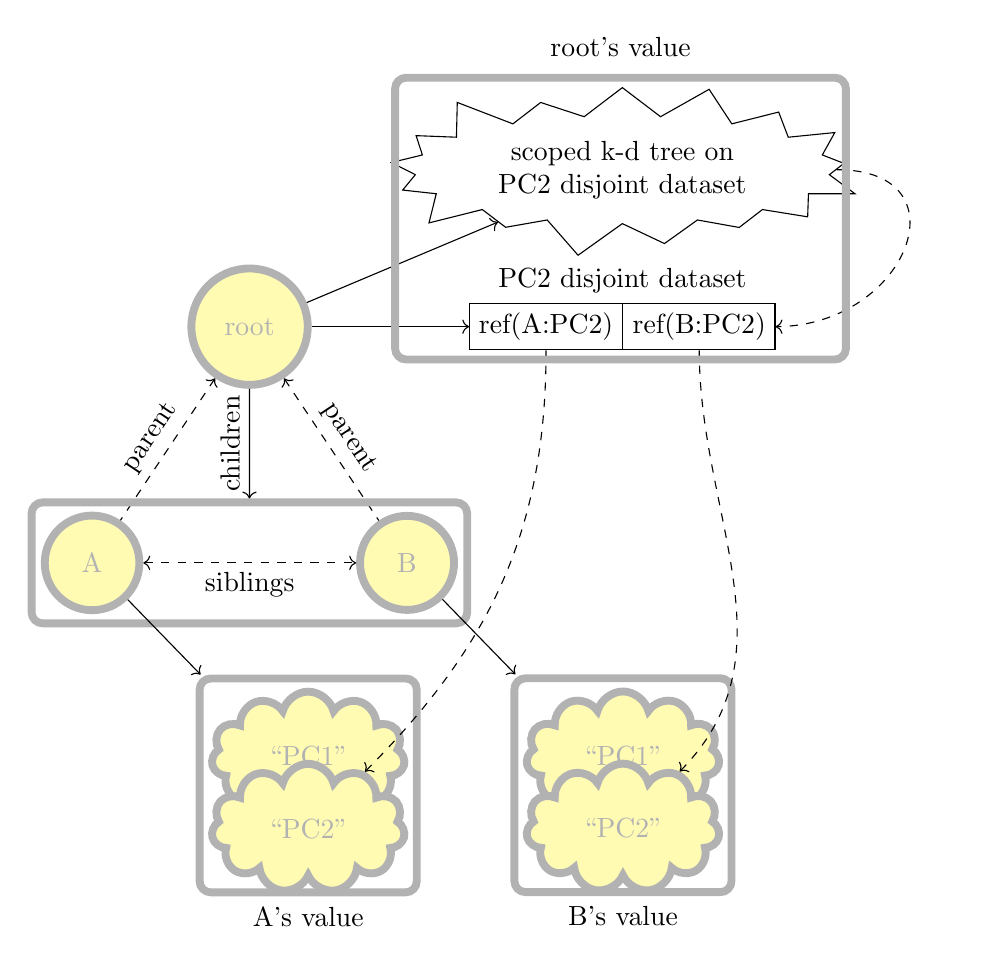
\begin{tikzpicture}[level/.style={sibling distance=40mm/#1}]
  \node[treenode] (r) {root}
  [level distance=30mm]
  child {
    node[treenode] (a) {A}
    edge from parent [<-,dashed]
    node[above,draw=none,sloped] {parent}
  }
  child {
    node[treenode] (b) {B}
    edge from parent [<-,dashed]
    node[above,draw=none,sloped] {parent}
  };
  \draw[dashed,<->] (a) -- node[below]{siblings} (b) ;

  \node[draw=black!30,line width=1mm,rounded corners,fit=(a) (b)] (children) {};
  \draw[->] (r) -- node[above,sloped]{children} (children);

  \pic (pcA) [below right=20mm of a] {namedpcs};
  \node[draw=black!30,line width=1mm,rounded corners,fit=(pcA-pc1) (pcA-pc2)] (aval) {};
  \draw[->] (a) -- (aval) ;
  \node[below=0.1mm of aval] {A's value};

  \pic (pcB) [below right=20mm of b] {namedpcs};
  \node[draw=black!30,line width=1mm,rounded corners,fit=(pcB-pc1) (pcB-pc2)] (bval) {};
  \draw[->] (b) -- (bval) ;
  \node[below=0.1mm of bval] {B's value};

  \node[disjointdataset=2,right=20mm of r] (djds) {
    ref(A:PC2)\nodepart{two}ref(B:PC2)};
  \draw[->] (r) -- (djds) ;
  \node[above=0.1mm of djds]{PC2 disjoint dataset};

  \node[starburst, draw, above=10mm of djds,align=center,text width=3.5cm] (kd) {
    scoped k-d tree on PC2 disjoint dataset};
  \draw[->] (r) -- (kd) ;

  \draw[dashed,out=45,in=-90,looseness=1,<-] (pcA-pc2) edge (djds.one south);
  \draw[dashed,out=45,in=-90,looseness=1,<-] (pcB-pc2) edge (djds.two south);
  \draw[dashed,out=0,in=0,looseness=2,->] (kd) edge (djds.two east);

  \node[draw=black!30,line width=1mm,rounded corners,fit=(djds) (kd)] (rval) {};
  \node[above=1mm of rval] {root's value};
\end{tikzpicture}
\end{center}



\end{document}
